\documentclass[problem]{mcs}

\begin{pcomments}
  \pcomment{MQ_matching_morning}
  \pcomment{by Peter (Jian) Huang 10/27/11, minor edit by ARM}
\end{pcomments}

\pkeywords{
  matching
  bipartite
  degree-constrained
  covers
}

%%%%%%%%%%%%%%%%%%%%%%%%%%%%%%%%%%%%%%%%%%%%%%%%%%%%%%%%%%%%%%%%%%%%%
% Problem starts here
%%%%%%%%%%%%%%%%%%%%%%%%%%%%%%%%%%%%%%%%%%%%%%%%%%%%%%%%%%%%%%%%%%%%%

\begin{problem}
The bipartite graph $H$ in Figure~\ref{fig:deg_constrained_bipartite}
has an easily checked property that ensures it has a \idx{matching} of
all the vertices in $\leftbi{H}$ with vertices in $\rightbi{H}$.
Verify that $H$ has this property---you do not need to find the
matching.

\begin{figure}[h]
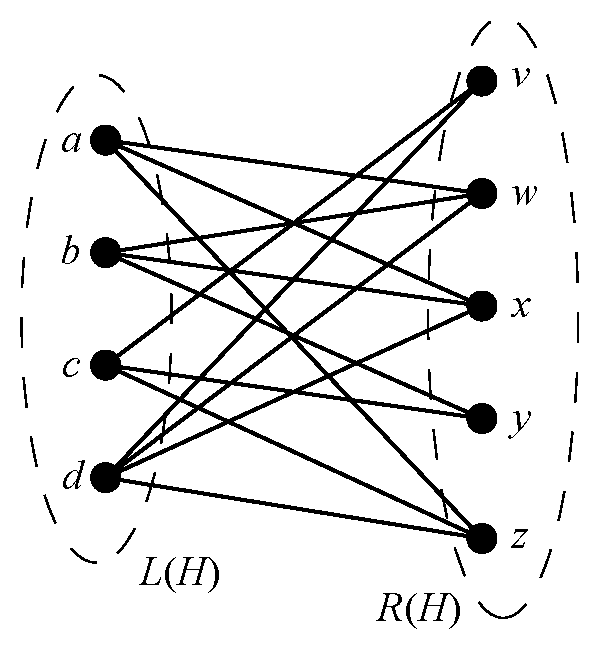
\includegraphics[width=2in]{MQ_degree_constrained_bipartite}
\caption{$H$.\label{fig:deg_constrained_bipartite}}
\end{figure}

\examspace[1in]
\begin{solution}
Each vertex in $\leftbi{H}$ has degree at least 3, while each vertex
in $\rightbi{H}$ has degree at most 3.  Consequently, the graph is
degree-constrained, which by
Theorem~\bref{lem:no_bottleneck_degree_constrained} implies there is a
matching that covers $\leftbi{H}$.

One matching, for example is:
\[
\edge{a}{z}, \edge{b}{w}, \edge{c}{v}, \edge{d}{x}.
\]
\end{solution}

\end{problem}

\endinput
